% This is lnicst.tex the demonstration file of the LaTeX macro package for
% Lecture Notes of the Institute for Computer Sciences, Social-Informatics 
% and Telecommunications Engineering series from Springer-Verlag.
% It serves as a template for authors as well.
% version 1.0 for LaTeX2e
%
\documentclass[lnicst]{svmultln}
%
\usepackage{graphicx} % includegraphics
\usepackage{makeidx}  % allows for indexgeneration
\usepackage{url} %for url citing
\usepackage{caption}
\usepackage[table]{xcolor}
\usepackage{listings}
\newcommand{\F}{Fig.}

\newcommand\DejaVuttfamily{%
  \fontfamily{DejaVuSansMono-TLF}\selectfont
}
\newcommand{\eg}{\textit{e}.\textit{g}.}
\lstset{
  language=C,numbers=left,xleftmargin=2.5em,
  basicstyle=\DejaVuttfamily\scriptsize,
  keywordstyle=\color{blue}\DejaVuttfamily,
  stringstyle=\color{red}\DejaVuttfamily,
  commentstyle=\color{Bittersweet}\DejaVuttfamily,
  moredelim=**[is][\color{red}]{@}{@},
  escapeinside={<@}{@>}
}
\usepackage{amsmath}
\usepackage{algorithm}
\usepackage[noend]{algpseudocode}

% \makeindex          % be prepared for an author index
%
\begin{document}
%
\mainmatter              % start of the contribution
%
\title{Obfuscation with Turing Machine}
%
\titlerunning{Turing Obfuscation}  % abbreviated title (for running head)
%                                     also used for the TOC unless
%                                     \toctitle is used
%
\author{Yan Wang \and Shuai Wang \and Pei Wang \and Dinghao Wu}
%
%\authorrunning{Wang et al.}   % abbreviated author list (for running head)
%
%%%% list of authors for the TOC (use if author list has to be modified)
\tocauthor{Yan Wang, Shuai Wang, Pei Wang, Dinghao Wu}
%
\institute{The Pennsylvania State University\\University Park, PA 16802, USA\\
\email{{ybw5084,szw175,pxw172,dwu}@ist.psu.edu} %\\ WWW home page:
%\texttt{http://users/\homedir iekeland/web/welcome.html}
% \and
% Universit\'{e} de Paris-Sud,
% Laboratoire d'Analyse Num\'{e}rique, B\^{a}timent 425,\\
% F-91405 Orsay Cedex, France}
}
\maketitle              
% typeset the title of the contribution
% \index{Ekeland, Ivar} % entries for the author index
% \index{Temam, Roger}  % of the whole volume
% \index{Dean, Jeffrey}

\begin{abstract}        % give a summary of your paper
Software security is a fundamental research domain in this threat emerging
technology world. Control flow obfuscation is one of the important techniques to
prevent hackers from understanding the program internal logic and leveraging
software vulnerabilities to do damage. Hence, concealing important conditional
branch logics are crucial for protecting software from being compromised. In
this paper, we propose a novel control flow obfuscation method by leveraging the
complexity of Turing machine. By entwining the original software programs with
Turing machine execution, control transfers could be selectively obfuscated.
Control flow graph and call graph could be significantly complicated. We
implemented an obfuscation tool named Turing machine obfuscator with LLVM.
Compared with previous works, our control flow obfuscation technique bears two
distinct advantages. 1). Complexity: Complicated implementation of Turing machine
makes it hard for attackers to follow the control flow graph
logic. 2). Universality: Our obfuscation happens on intermediate representative
level so the application scope is broadened to almost every language with an LLVM
front-end compiler. We evaluate the obfuscator by potency, resilience, stealth,
and cost, respectively. Experimental results show that Turing machine obfuscator
could obfuscate programs in stealth with good performance and robustness.
%please supply keywords within your abstract
\keywords {software security, control flow obfuscation, Turing machine, LLVM}
\end{abstract}
%
\section{Introduction}
\label{sec:introduction}
Obfuscation derives from intellectual property protection. The Internet brings
us unprecedented convenience along with idea plagiarism threat and copyright
infringement. Concealing the algorithm of a software means a lot for the society
especially for high-tech industry. Attackers could take advantage of the
state-of-the-art techniques~\cite{Loop,Lee,Molnar} to recover source code
structure from binaries, exploit software vulnerabilities or to steal software
ideas or algorithms. Obfuscation is mostly designed to impede such (malicious)
reverse engineering process.

Recently, Software security research again draws people's attention because of
infamous ransomware attack and severe vulnerabilities such as the ``Wanncry''
incidence and the OpenSSL heart bleeding bug. All of these malwares exploit
vulnerabilities inside a software. To exploit vulnerabilities in the software,
attackers usually need to recover the program control-flow structures first.
Dynamic code analysis is a popular and effective technique to explore inner
logic of a program. \textit{Concolic testing} is well-developed and
widely-adopted technique which leverages both symbolic and concrete execution to
cover all the program paths\cite{Sen}. 
The concolic
testing engines like SAGE\cite{Sage} and KLEE\cite{klee} could yield new input which leads to a new execution path by solving
path conditions as constraints based on previous execution. 
It has been proved effective in analysing control flow graph(CFG) of software\cite{Cute}.

Hence, a lot of anti-reverse engineering research has focused on preventing
adversaries from analyzing important path conditions in a
program\cite{Opaque,Sharif,Popov,Zhi, Wang:Zhi}. Control flow obfuscation is one
of these cutting-edge techniques to combat these reverse engineering tools.
Control flow obfuscation aims at hiding path conditions and complicating the
execution flow within a program. By rewriting or adding extra control flow
components, the program path conditions become difficult or even impossible to
analyze. Existing research \cite{Ma} have demonstrated the effectiveness of
control flow obfuscation.

% \begin{figure}
%   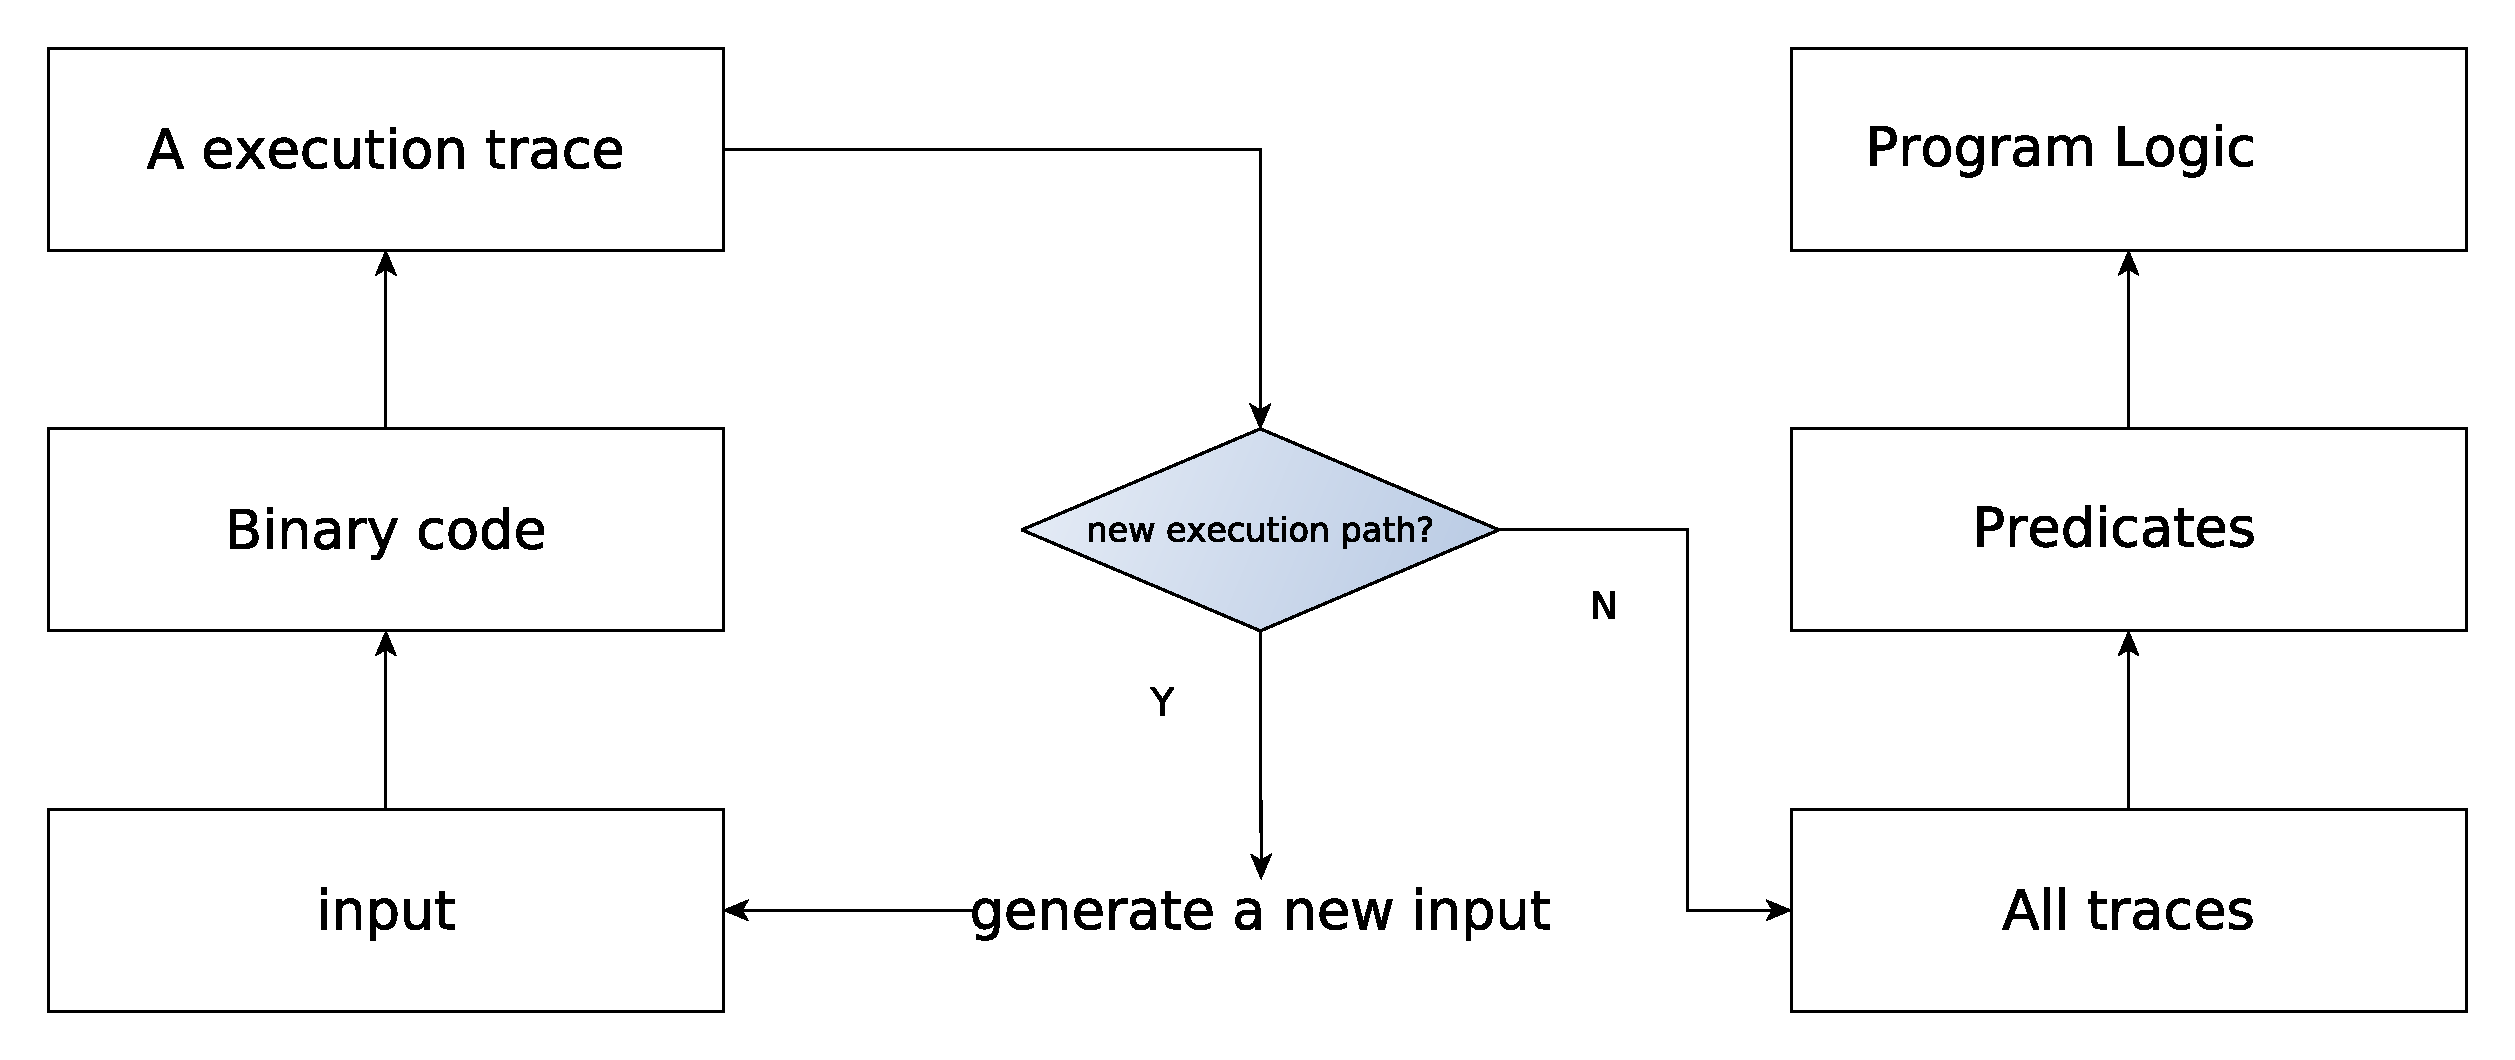
\includegraphics[width=0.9\linewidth]{reverse_engineering.eps}
%   \caption{Reverse engineering with concolic testing}
%   \label{fig:one}
% \end{figure}

In this paper, we propose a novel control flow obfuscation method which
leverages Turing machine to compute path conditions. \textit{Church---Turing
  thesis} has shown that any function is computable by a human being without
resource limitation concerns if and only if this function is computable by a
Turing machine~\cite{Church}. This means any functional component of software
can be re-implemented as a Turing machine; the replaced code component and its
corresponding semantic equivalent Turing machine is called \textit{Turing
  Equivalent}.

In this work, we propose to simulate important branch conditions in original
source code with its \textit{Turing Equivalent} Turing machine. A Turing machine
behaves as a state machine so it would bring in a large amount of extra control
flow transfers and basic blocks to the overall program control flow graph. A
typical Turing machine leverages transition tables to guide the state
transition, and such transition table-based execution would introduce additional
computations to the target program. We believe the proposed Turing machine
obfuscation would largely complicate the protected program, and also bring in
new challenges for reverse engineering tasks.

To obfuscate a program through the proposed Turing machine obfuscation
technique, we first translate the original program source code into a compiler
intermediate representation. Our Turing machine obfuscator then selects path
condition instructions for translation; the translated instruction will invoke
its corresponding Turing machine component, which is semantically equivalent to
the original path condition. After finishing the execution in the Turing machine
``black box'', the execution flow returns back to the original instruction, with
a return value that indicates the branch selection. Inspired by previous
work~\cite{Collberg}, we evaluate our obfuscator regarding four aspects which
are potency, resilience, cost and stealth, respectively. Results indicate that
Turing machine obfuscator could effectively obfuscate commonly-used software
with acceptable performance penalty.

This paper is organized as follows. Section 2 discusses related works on
obfuscation, especially control flow obfuscation. Section 3 presents the overall
design of Turing machine obfuscator. Obfuscator implementation is discussed in
section 4. Section 5 presents the evaluation result of our proposed technique.
We further present discussion in section 6, and conclude the paper in Section 7.


%
\section{Related Work}
%
Generally speaking, reverse engineering techniques are categorized into static
track and dynamic track. To battle static reverse engineering, researchers
usually focus on hardening disassembling and decompiling process. To combat the
dynamic reverse engineering techniques such as concolic testing, sensitive
conditional transfer logic must be hidden from adversaries. Control flow
obfuscation has been proved effective in this scenario.

Sharif et al. (\cite{Sharif}) identify conditions that could trigger malware
execution then using a hash function to transform such condition outputs. Hence,
corresponding conditional codes which would be run with the trigger value were
encrypted with a key generated based on the instruction trigger value. By this
means the obfuscation analyzer could never get a chance to get the expected
``launching code'' consequently planted malware could never be executed. This
technology works on certain fixed trigger value but not in scenarios that
trigger values are intervals. This limitation narrows the application scopes
greatly since a large volume of branch conditions are comparison operations. In
addition, the encryption and decryption process in this methodology also
introduce non-negligible overhead.

Popov et al. (\cite{Popov}) propose to leverage signals (``traps'') to replace
the unconditional control transfer instructions such as \texttt{jmp} and
\texttt{call} to impede disassembly operation which is the first step of reverse
engineering. Moreover, dummy control transfers and junk instructions are also
inserted after signal replacements. This method seems to be effective in fooling
disassemblers but it cannot be applied in scenarios that the conditional control
flow transfers need to be protected.

Another related work proposes to cover branch information leveraging a remote
trusted third party environment~\cite{Zhi}. In general, their technique mostly
introduces notable network overhead and also relies on trusted network
accessibility which may not be feasible in practice. 

Ma et al. (\cite{Ma, Maieee}) take advantage of neural network to replace
certain branch condition statements in source programs; the propose technique is
evaluated to conceal conditional instructions and dynamic analysis such as
concolic testing would be trapped to cover the protected branches. Although the
idea is promising and the experimental results indicate the effectiveness to
certain degree, in general neural network-based solution may not be suitable for
such scenarios. To the best of our knowledge, neural network works like a black
box; it lacks a rigorous theoretical foundation to show a correct result can
always to generated given an input. In other words, neural networks may yield
results which lead to the selection of incorrect branches. Overall, neural
networks not only introduce complexity but also unpredictability to the
transformed programs. Trained models may behave very differently if given
initial parameters with only some nuances, which means that it is very
challenging to train an accurate enough model to simulate the conditional
instruction. In addition, we notice that neural network usually consumes too
much memory in the evaluations.

%
\section{Turing machine obfuscation}
%
\subsection{Design Overview}
In a program, a path condition statement compares two operands and selects a
branch for control transfer based on the comparison result. In theory, Turing
machine has been proved to be able to simulate the semantics of any computer
algorithm. Hence, any program path condition statement can be modeled by a
Turing machine. Taking advantage of its powerful computation ability as well as
execution complexity, we propose to employ Turing machine to obfuscate path
condition statements in a program. The general workflow of a Turing machine
obfuscated path condition statement is shown in \F~\ref{fig:two}. As shown in
the figure, instead of directly computing a boolean value in the condition
statement, we feed a Turing machine with the inputs (the value of operands) and
let the Turing machine to simulate the execution.

\begin{figure}
 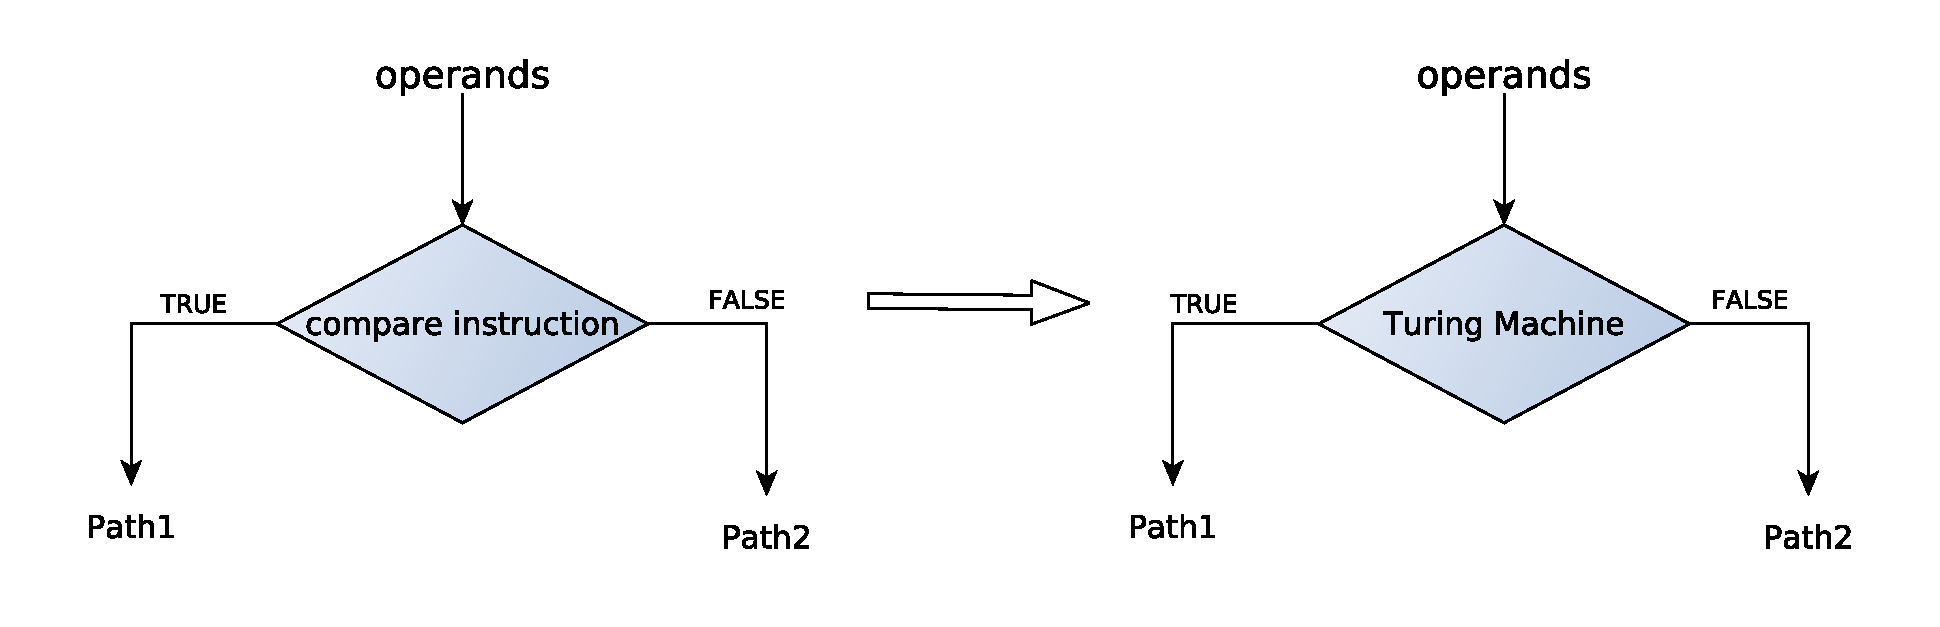
\includegraphics[width=\linewidth]{figure2.eps}
 \caption{Obfuscate a path condition statement through a Turing machine.}
 \label{fig:two}
\end{figure}

\subsection{Turing Machine}
Turing Machine is a mathematical model which could simulate any computer
program. As shown in \F~\ref{fig:three}, a typical Turing machine consists of
four components:
\begin{itemize}
  \item An infinite-long tape which consists of a sequence of cells. Each cell
    holds a symbol defined in the tape alphabet. In implementation,  Turing machine obfuscator dynamically allocates new
  tape cells to construct an infinite tape used to store intermediate results.
  \item A tape head which could conduct read, write, move left and move right
    operations.
  \item A state register used to record the state of the Turing machine. Turing
    machine states are finite.
  \item A transition table that consists of all the transition rules defining
    how a Turing machine transfers from one state to another.
\end{itemize}

\begin{figure}
 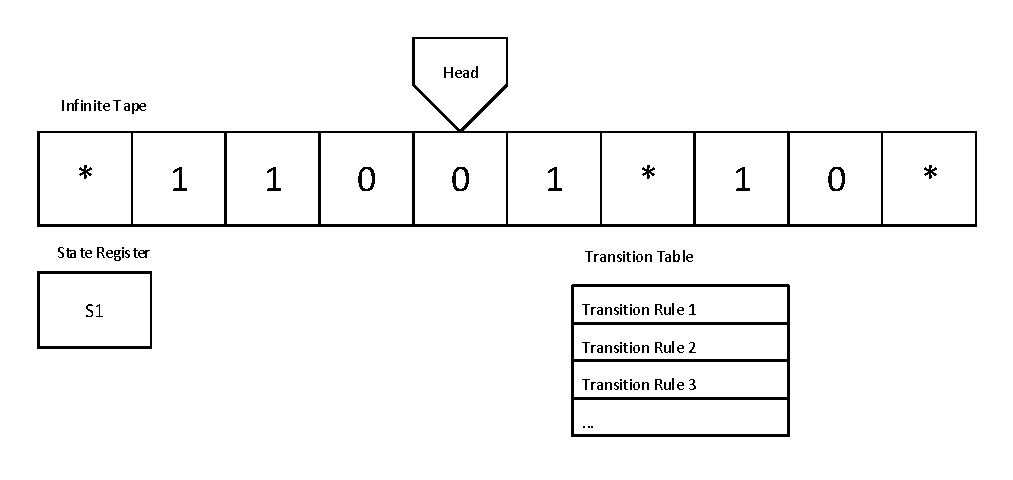
\includegraphics[width=0.9\linewidth]{TM.pdf}
 \caption{Turing Machine Components}
 \label{fig:three}
\end{figure}


% Formally a Turing machine could be represented by a 7 element tuple\cite{Turing}: \[ (Q, \Gamma, b, \Sigma, \delta, q_0, F) \] 
% where:
% \begin{itemize}
%   %\renewcommand{\labelitemi}{$\star$}
%   \item \(Q\) is finite state set
%   \item \(\Gamma\) is finite tape symbol set named alphabet
%   \item \(b\) is the tape blank symbol. \(b \in \Gamma\)
%   \item \(\Sigma \subset \Gamma \)\textbackslash  \(\{b\}\) is the actual input symbol set without blank symbol
%   \item \(\delta\) is the transition table composed of transition rules in form of \((Q\)\textbackslash \(F)\times\Gamma \rightarrow Q \times \Gamma \times \{L,R\}\) 
%   \item \(q_0 \in Q \) is the initial state
%   \item \(F\) is finite acceptable states set. \(F \subset Q\)
% \end{itemize}

\subsubsection{Transition Table}
Mathematically a transition rule could be represented by a 5 element
tuple:\[(S_c, T_c, S_n, T_n, D)\] where:

\begin{itemize}
  \item \(S_c\) is the current Turing machine state
  \item \(T_c\) is the current tape cell symbol read by the head
  \item \(S_n\) is the new Turing machine state
  \item \(T_n\) is the symbol head writes to current tape cell
  \item \(D\) is the direction the head should move (i.e., ``left'' or
    ``right'')
\end{itemize}

Every 5 element tuple represents a transition table rule in \ref{fig:three}.
Although simple, Turing machine model resembles a modern computer in several ways. 
The head is I/O device. The infinite tape acts as the computer memory.
The transition table defines the mission of this Turing machine which is like program
code and data. Hence, Turing machine is also deemed as
the foundation of modern computer science development.


\subsubsection{Turing machine initialization}

Initially, Turing machine is in ``start'' (\(S_0\)) state and tape records the
Turing machine input. Blank symbol is symbolized as Char ``*'' on tape.
Consistent with existing Turing machine simulator project~\cite{SingleTape}, we
use the length of ``$\cdot$'' to represent an operand of integer type. For
instance, integer 5 is represented as five continuous ``$\cdot$'' on tape.
Turing machine tape alphabet is $\{\cdot,* \}$. The tape in \F~\ref{fig:three}
displayed an initial state of Turing machine. The head of Turing machine is
placed on the leftmost cell. Different integer operands are separated by a
single blank symbol ``*''. Operands encoded on the tape of
  \F~\ref{fig:three} are 5 and 1. When Turing machine starts to run, the head
reads the current tape cell, combining with current state register value it
could locate one and only one match transition rule in the transition table. This matched 
transition rule entry will direct Turing machine to change to next step.


\subsubsection{Turing machine running}
The Turing machine keeps running step by step directed by the transition table
until it reaches a \texttt{Halt} state. On the other hand, Turing machine may
keep running forever since the process of solving some problems cannot
terminate. In our research, we implement Turing machine to do simple algebra
computations so it would always reach a \texttt{Halt} state. When reaching the
\texttt{Halt} state, the machine stops running and the computation result is
shown on the tape. Table~\ref{table:1} shows a transition table example, which
supports a Turing machine to conduct the \texttt{add} operation in our
implementation.

\begin{table}
\centering
\begin{tabular}{ |c|c|c|c|c|} 
  \hline
  \textbf{Current State} & \textbf{Current Symbol} & \textbf{New State} & \textbf{New Symbol} & \textbf{Direction} \\ 
  \hline
  \(S_0\) & * & \(S_0\) & * & Right\\ 
  \hline
  \(S_0\) & . &\(S_1\)  & . & Right\\
  \hline
  \(S_1\) & * &\(S_2\) & . & Right\\  
  \hline
  \(S_1\) & . & \(S_1\) & . & Right \\
  \hline
  \(S_2\) & * & \(S_3\) & * & Left \\
  \hline
  \(S_2\) & . & \(S_2\) & . & Right \\
  \hline
  \(S_3\) & * & \(S_3\) & * & Left \\
  \hline
  \(S_3\) & . & \(S_4\) & * & Left \\
  \hline
  \(S_4\) & * & \(Halt\) & * & - \\
  \hline
  \(S_4\) & . & \(S_4\) & . & Left\\
  \hline

\end{tabular}
\caption{Transition table of the \texttt{add} operation in a Turing machine.}
\label{table:1}
\end{table}

\subsubsection{Addition Turing Machine}

In this section, we elaborate the design of ``add'' Turing machine which
simulates the semantics of the addition operation. Other Turing
  machines(\texttt{substractiong} Turing machine, \texttt{multiplication} Turing machine and \texttt{division} Turing machine) used in this research are designed in a similar way.
  Through constructing this transition table, we essentially
  build rules which could concatenate two integer dot cells together. 
  Take initial tape in \F~\ref{fig:three} as an example. Following the rules in table \ref{table:1}, after a
  sequence of reading and writing operations based on the transition table, left operand 5 and right operand 1(enbodied by two series of
  operand dot cells) which are splited by \textit{blank symbol} ``*'' are merged into a long series of dot cells on tape; the length of
  outcome dot cells is the sum of two operands 6 as shown in \F~\ref{fig:turing_outcome}. 

\begin{figure}
 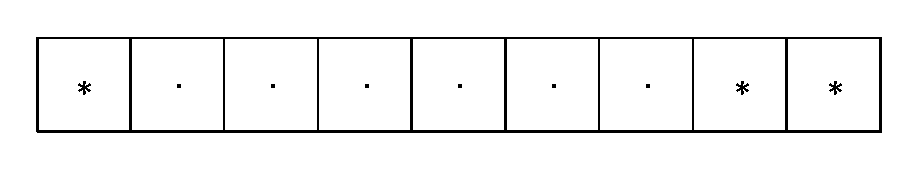
\includegraphics[width=0.9\linewidth]{Turingaddoutcome.pdf}
 \caption{Turing machine execution result}
 \label{fig:turing_outcome}
\end{figure}

Adding Turing Machine Transition table encodes the running algorithm which is
simplified in Algorithm~\ref{adding}. Algorithm~\ref{adding} in fact states a
method how to combine two series of dot cells on tape together. Following the
algorithm, the isolator cell \textit{blank symbol} is erased when Turing machine
finally enter the ``Halt'' state.


  % When Turing machine completes execution process, the sum of left and right
  % operand is yield on the tape. The length of the result is exactly the sum of
  % two operands because Turing machine erase one dot cell of right operand and
  % complement with one dot cell between the two input operands.

\begin{algorithm}
\caption{Transition table algorithm for the ``add'' Turing machine.}
\label{adding}
\begin{algorithmic}[1]
\Procedure{running procedure}{}
\State $\textit{head} \gets \text{blank cell before left operand starting cell}$
\While{$\text{head}$ != blank cell after right operand}
 move right\;
\EndWhile

\State move left
\State $\text{last dot cell of right operand} \gets \text{blank symbol}$

\While{$\text{head}$ != blank cell isolator of two operands}{
  move left\;
}
\EndWhile
\State $\text{blank cell isolator} \gets \text{dot}$
\While{$\text{head}$ != blank cell befor left operand}
  move left\;
\EndWhile
\State \textbf{Halt;}
\EndProcedure
\end{algorithmic}
\end{algorithm}
`
\subsubsection{Turing Machine of other operations}
As previously discussed, given any program algorithm, there must exist a
corresponding Turing machine. Since our Turing machine obfuscator concentrates
on obfuscating conditional branch instruction with arithmetic operations(\eg\lstinline{if(a*b>c)... }), Turing
machine obfuscator need to contain transition tables which is capable of doing
arithmetic operations such as \(+, -, \times, \div\).

To implement the arithmetic operations, besides the addition transition table shown in
Table~\ref{table:1}, we construct three more tables for subtraction,
multiplication and division operations. Their transition tables are relatively
more complex than Table~\ref{table:1}. Actually in our implementation, we build
transition table consisting of 16, 34 and 80 transition rules entries for subtraction,
multiplication and division Turing machines, respectively.
As for the comparison operations such as \(\leq, \geq, \neq\) between operands, we take advantage of 
subtraction Turing machine to calculated the difference of them. Based on calculation result, \lstinline{True/False} is 
returned. In sum, we construct 4 transition tables, with overall 140
  transition table entries.



\subsection{Universal Turing Machine}
While a Turing machine could perform powerful algorithm simulation, its
computation ability is predetermined by its initial tape state and embedded transition table. For
instance, a Turing machine capable of doing addition operation could only
simulate the ``add'' operation since other operations would have very distinct
transition rules. A ``add'' Turing machine could not represent ``subtract''
operations. A Turing machine encoded with 2 + 3 could not conduct addtion operation 5 + 6.
To some degree, each Turing machine is encoded with a fixed
algorithm and input data. However, in non-trivial programs, path condition operands could be any kind
of operation such as \(x + 5\) or \(6 \times 7 \). Many of these algebra
expressions would correspond to different Turing machines. Hence, we need an
unified translator to represent arbitrary computations. Universal Turing machine
is designed to simulate arbitrary Turing machines. It stores and interprets
arbitrary a Turing machine on a single tape. As shown in \F~\ref{fig:four}, both
input data and transition table are written on the tape of the universal
Turing machine. In some sense, a universal Turing machine acts as the interface
for us to employ Turing machines of different semantics.


Universal Turing machine bears the essence of the modern computer which is being
programmable. Through storing different transition tables on a sequence of cells
on the tape, an universal Turing machine can actually perform semantic
equivalent computation to arbitrary programs; as aforementioned, such Universal
Turing Machine and the replaced algebra expression are \textit{Turing
  Equivalent}. In our Turing machine obfuscator, we can invoke a Universal
Turing machine function call on interested conditional control transfer instructions and related arithmetic operation
instructions.


\begin{figure}
 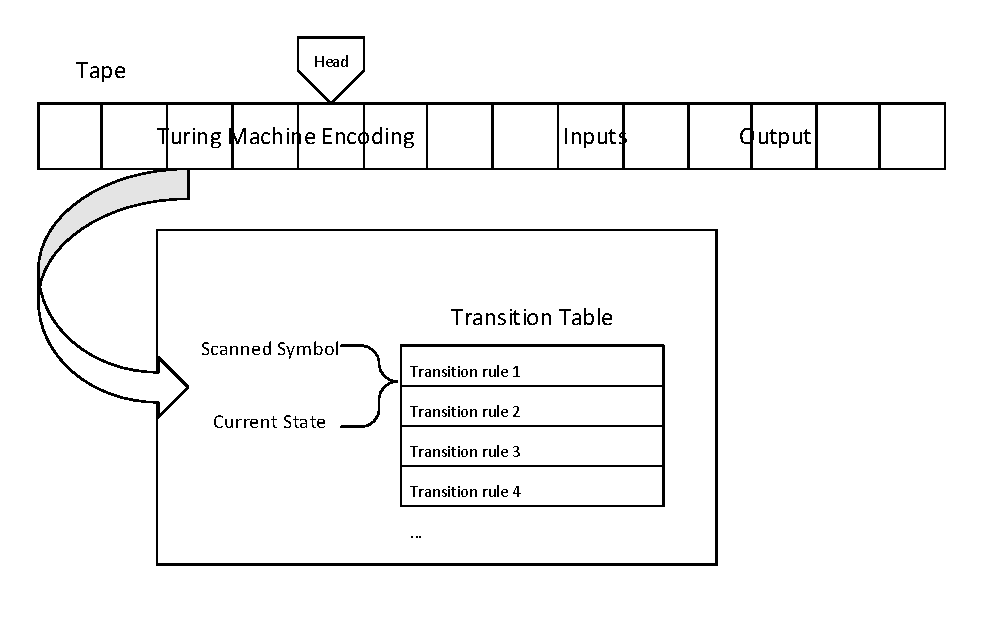
\includegraphics[width=\linewidth]{UTM.pdf}
 \caption{Overall workflow of a universal Turing machine.}
 \label{fig:four}
\end{figure}

\subsubsection{Tape construction}
Before universal Turing machine execution, a tape which contains the input
operands and Turing machine transition tables is generated. For each operation
of ``\(+\)'', ``\(-\)'', ``\(\times\)'' and ``\(\div\)'', corresponding
transition table is also embedded on tape. As aforementioned, integer inputs are
encoded as strings of ``.'' with different lengths. Following a universalized
tape formatting protocol across Turing machine obfuscator, we concatenate
transition tables and inputs to form a tape for the universal Turing machine. In
this way, all the information needed for computations exists on the tape. During
the execution of universal Turing machine, it would first extract a proper
transition table then perform one step computation.

\subsubsection{Negative Integer Operand Preprocess}
% what if 4 + (-6)?  would you translate it into 4 + 6?
\textcolor{red}{still not clear}
In software programs, integer operands comprise both positive and negative
cases. Turing machine could only dispose of positive operands in consequence of
we use the length of dot cell on tape to represent a integer. This means we have
to preprocess the invalid operands in Turing machine obfuscator. In the
preprocessing stage, Turing machine obfuscator could convert invalid operands to
its opposite number to run Turing machine. Calculate result from Turing machine
is also revised before returning. For instance, $-4 + (-6)$ is preprocessed to
$4 + 6$, afterwards -10 which is the opposite number of 10 is returned. $4 +
(-6)$ is preprocessed to Turing machine operation $6 - 4$, and the opposite
number of the outcome 2 (i.e., -2) is returned. In preprocess stage, any
arithmetic operation would be transformed to a valid integer operation with $+$,
$-$, $\times$, $\div$ for Turing machine.

\section{Implementation}
Our proposed technique is implemented as a transformation pass of the LLVM
compiler suite~\cite{LLVM}; the LLVM intermediate representation (IR) is
obfuscated and then compiled into binary executable. As shown in
\F~\ref{fig:five}, our Turing obfuscator performs a three-phase process to
generate the obfuscated output. The first step translates both target program
and obfuscator's source code into LLVM IR. The obfuscator then iterates IR
instructions to identify obfuscation candidates and perform the transformation.
The instrumented IR codes are further compiled into the executable file in the
final step. \textcolor{red}{We implement the Turing machine obfuscator in C,
  with in total XXX lines of code}.

\begin{figure}
 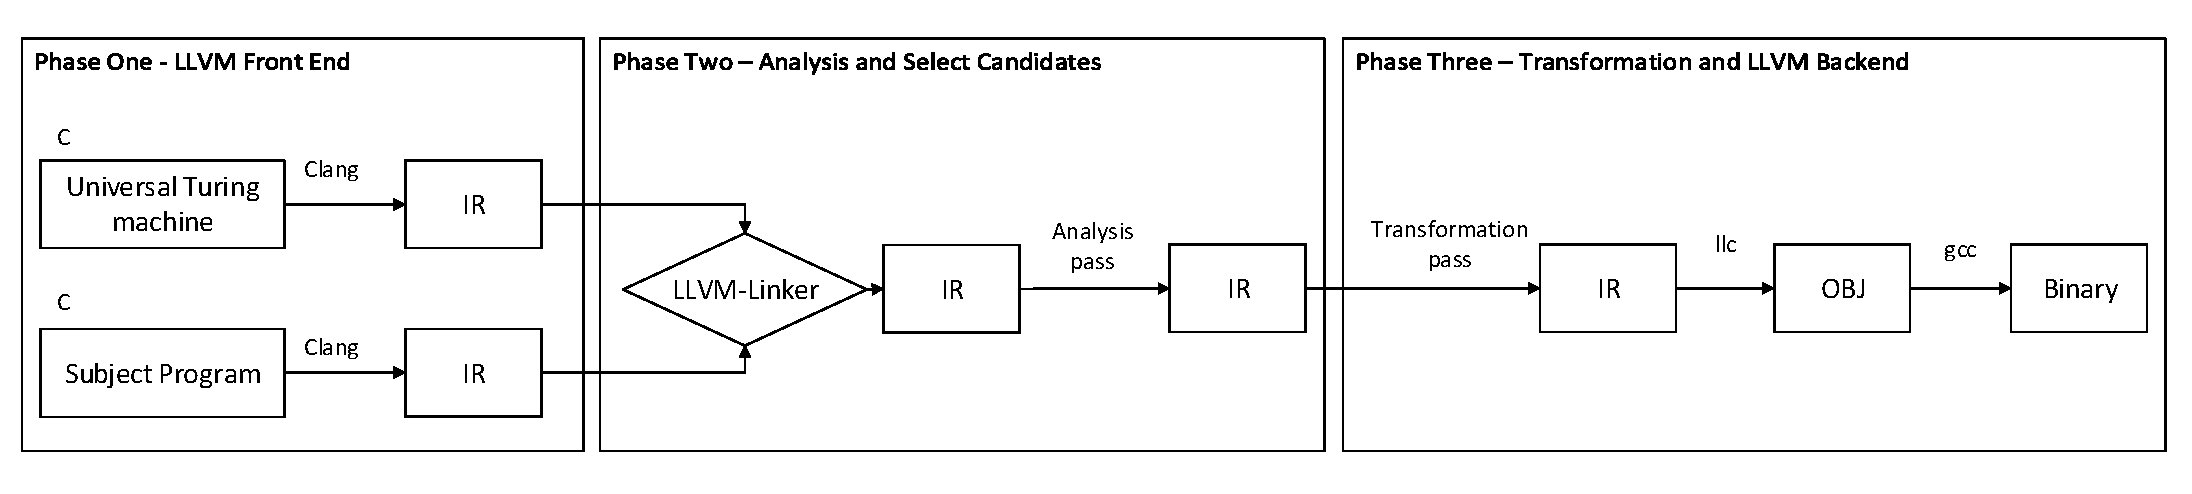
\includegraphics[width=\linewidth]{overview.pdf}
 \caption{Workflow of Turing machine obfuscator.}
 \label{fig:five}
\end{figure}

\subsection{Phase One: Translating Source Code to IR}
\label{subsec:phase-one}
As aforementioned, we first compiles the target source program into LLVM IR; the
obfuscation transformation is performed on the IR level. Considering a broad set
of front end compilers provided by LLVM which can turn programs written by
various programming languages into LLVM IR, this IR-based implementation could
broaden the application scope our tool comparing with previous
work~\cite{Ma, Zhi, Maieee}. On the other hand, since we employ C programs for
the evaluation, Clang (version 5.0) is used as the front end compiler in this
paper.

\subsection{Phase Two: Collect Transformation Candidate}
During the static analysis pass, our Turing machine obfuscator locates all
transformation candidates on the IR instructions. The LLVM Pass framework is a
core module of the LLVM compiler suite to conduct analysis, transformation and
optimization during the compile time~\cite{llvmpass}. We build a extra pass
within this framework to iterate and analyze every IR instruction in each module
of the input program. 
\\\\
\noindent \textbf{Locate Candidate Predicates} While the proposed technique is
fundamentally capable of obfuscating any program component, the implementation
currently focuses on branch predicate since control-flow obfuscation is
efficient to defeat many reverse engineering activities
(\S~\ref{sec:introduction}). In general, the transformation candidate set
includes instructions to compute different branch predicates (in total 10 kinds)
such as: equal, not equal, less than, greater than. \textcolor{red}{integer
  predicate}

\subsection{Phase Three: Transformation Pass}
The second phase provides all the eligible transformation candidates. In this
step, we build another transformation pass within the LLVM Pass framework to
perform the obfuscation transformation. As shown in \F~\ref{fig:six}, predicate
instructions are obfuscated; we rewrite the instructions into function calls to
the universal Turing machine interface. The computation of the branch predicate
is launched inside the Turing machine, and the computation result is passed to a
register which directs the associated path selection. The essence of Turing
obfuscator is to hide program control transfers; our technique is able to
obfuscate all the branch predicates in a program or only transform a subset of
(security sensitive) candidates. Such partial obfuscation is denoted as
``obfuscation level'' and we present discussion on this shortly.

\begin{figure}
 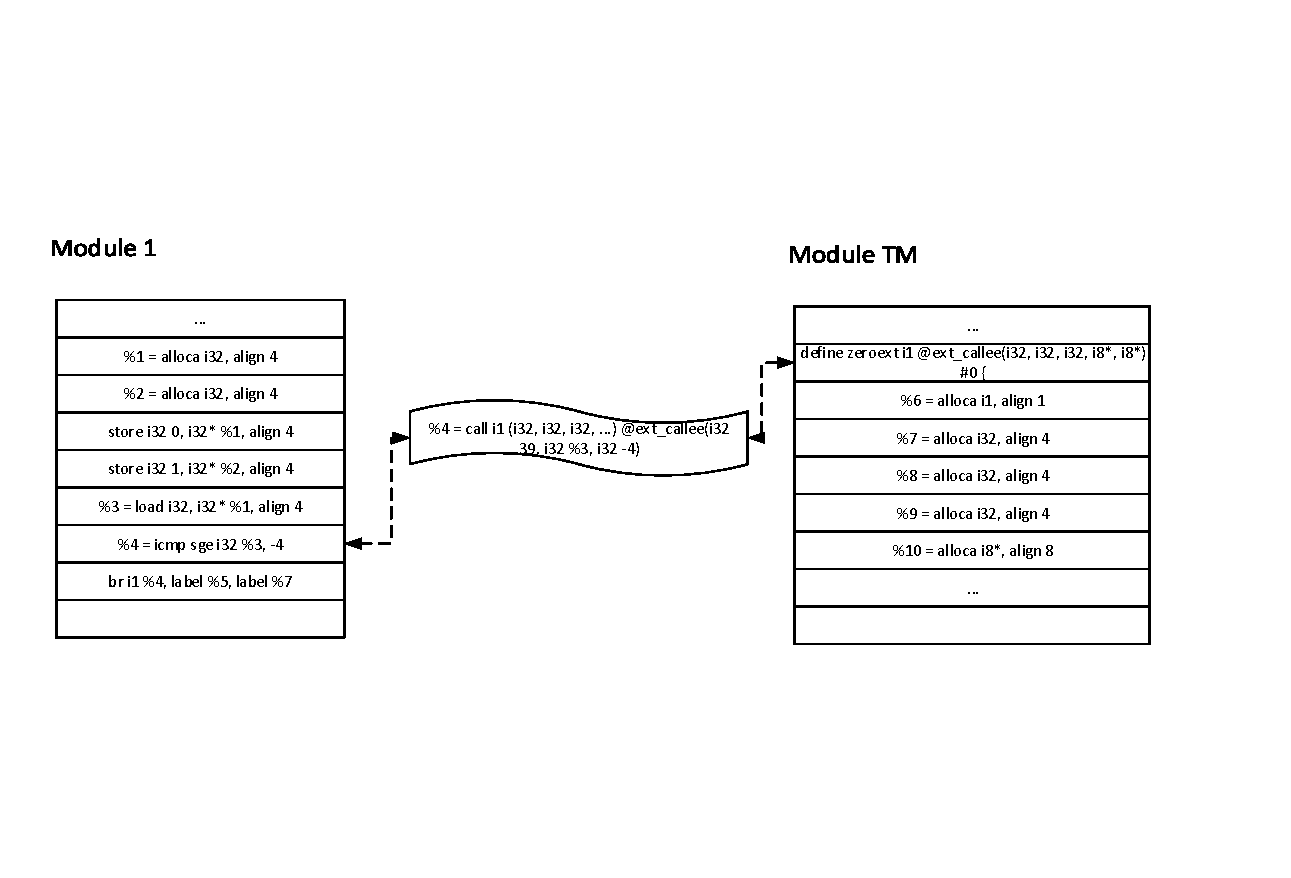
\includegraphics[width=\linewidth]{transform_pass.pdf}
 \caption{Phase Three: Transformation Pass}
 \label{fig:six}
\end{figure}

For an obfuscated predicate, our current ``transform to function call''
implementation utilizes the boolean return value to select a branch for control
transfer. On the other hand, we notice existing work (e.g., \cite{Ma, Maieee})
leverages a cross-procedure jump at this step; an indirect jump from the black
box of the Turing machine to a selected branch. We present further discussion on
both branch determination strategies in \S~\ref{sec:discussion}.
%% We also notice that if obfuscation could cover branch information further if we
%% could jump back to a caller function basic block based on the Turing machine
%% running result like in \cite{Ma}, but essentially it still expose branch trace
%% since we need to record the basic block addresses of each branch. To the best of
%% our knowledge, perfecting branch hiding technique does not exist since there is
%% always a way to figure out inner logic of a certain program given enough time
%% and energy. We need to harden this process as much as possible. Currently we
%% adopt the IR replacement way to invoke Turing machine.
\\\\
\noindent \textbf{Obfuscation Level} Obfuscation level is an indicator which
weighs how much of a program is transformed by the obfuscation pass. Consistent
with previous work (\cite{Trans}), the obfuscation level is defined as the ratio
between the obfuscated instruction and total eligible candidates:

\[ O = M / N \]

\begin{itemize}
  \item \(M\) is the number of instructions transformed by the obfuscation pass.
  \item \(N\) is the number of all the transformable instructions (i.e., the
    branch predicate instructions identified in \S~\ref{subsec:phase-one}).
\end{itemize}

\section{Evaluation}
\label{sec:evaluation}
Inspired by previous research~\cite{Collberg, Ma, Maieee}, we evaluate our
Turing machine obfuscator based on four metrics which are \textit{potency},
\textit{resilience}, \textit{stealth} and \textit{cost}, respectively. Potency
weighs the complexity of the obfuscated programs, which is straightforward to
show how competent an obfuscator is. A good obfuscator also needs to protect
itself from being deobfuscated; to measure how well an obfuscated program is
resilient to automatic deobfuscation techniques, we evaluate the resilience of
our Turing machine obfuscator. Moreover, in the battle against experienced
attackers, obfuscated programs should not be too distinguishable from its
origins otherwise it would be easy to be recognized. Hence, we measure the
stealth to show how well an obfuscated program resembles the original one. Cost
is naturally employed to measure the execution overhead of a software program.
While obfuscation would inevitably introduce performance penalty, we measure the
execution time of the obfuscated code to show the overall cost is acceptable.

Two widely-used open source programs are employed in our evaluation: compress
tool \textsc{bzip2}~\cite{bzip2} and regular expression engine slre~\cite{slre}.
In Turing machine obfuscator, we collect all path conditional branch instructions (e.g.,
\texttt{icmp}). Through \textit{Use-Define chain}, we also locate all  instructions that determine the value of the
conditional branch instruction, all these instructions are deemed as
transformation candidates. Obfuscation level is an index which represents the
ratio between obfuscated instructions and all candidates. In our experiments,
the ratio is set as 50\% which means half of all conditional transfer candidates
are \textit{randomly} selected and obfuscated.

%%%%%%% BY saying conditional *transfer* instruction, you mean the ``jump''
%%%%%%% instruction??  I mean the conditional branch instruction such as "icmp"

\subsection{Potency}
%
Control flow graph (CFG) and call graph provide insights on the general
structure of a program and they are the foundation for most static software
analysis. With the help of IDA Pro~\cite{ida} which is a well-known commercial
disassembler and debugger, we recover CFG and call graph information from both
original and obfuscated binaries. By traversing the graph, we further calculate
the number of basic blocks, number of call graph and control graph edges. We use
such information to measure the complexity of a program, which is aligned with
previous research~\cite{Chen}. Analysis result are shown in Table~\ref{tab:two}.
Comparing the original and obfuscated programs, it can be observed that program
complexity is increased in terms of each metric.

\begin{table}
  \centering
 \caption{Potency evaluation in terms of program structure-level information.}
 \label{tab:two}
 \begin{tabular}{|c|c|c|c|}
 \hline 
 \textbf{Program} & \textbf{\# of CFG Edges} & \textbf{\# of Basic Blocks} & \textbf{\# of Function} \\
 \hline
\textsc{bzip2} & 3942 & 2647 & 78 \\ 
 \hline
obfuscated \textsc{bzip2} & 4195 & 2828 & 134 \\
 \hline
\textsc{regexp} & 906 & 619 & 25 \\ 
 \hline
obfuscated \textsc{regexp} & 1122 & 773 & 43 \\
 \hline
\end{tabular}
\end{table}

We further quantify the Turing machine obfuscated programs w.r.t. the cyclomatic
number and knot number (these two metrics are introduced in
\cite{McCabe,Woodward}). Cyclomatic metric is defined as \[ Cyclomatic = E - N +
2 \] where E and N represent the number of edges and the number of nodes in a
CFG, respectively. Knot number shows the number of edge crossings in a CFG.
These two metrics intuitively weighs how complicated a program is in terms of
logic diversion number. Results in Table~\ref{tab:three} shows that both knot
number and cyclomatic number notably increase after Turing machine obfuscation.
Overall, we interpret Table~\ref{tab:two} and Table~\ref{tab:three} as promising
results to show program becomes more complex after the Turing machine
obfuscation.

\begin{table}
  \centering
 \caption{Potency evaluation in terms of knot and cyclomatic number.}
 \label{tab:three}
 \begin{tabular}{|c|c|c|}
 \hline 
 \textbf{Program} & \textbf{\# of Cyclomatic} & \textbf{\# of Knot} \\
 \hline
\textsc{bzip2} & 1297 & 5596  \\ 
 \hline
obfuscated \textsc{bzip2} & 1369 & 5720  \\
 \hline
\textsc{regexp} & 289 & 478 \\ 
 \hline
obfuscated \textsc{regexp} & 351 & 1068 \\
 \hline
\end{tabular}
\end{table}

Besides picking 50\% as the obfuscation level in evaluating potency, we also
conduct experiments with obfuscation levels as 30\%, 80\% and 100\%.
\F~\ref{fig:seven} shows the number of call graph edges regarding different
obfuscation levels. Observation shows that with a higher obfuscation level, the
number of call graph edge increases. We interpret the results that the
obfuscated program become more complicated with the obfuscation level increases.

\begin{figure}
  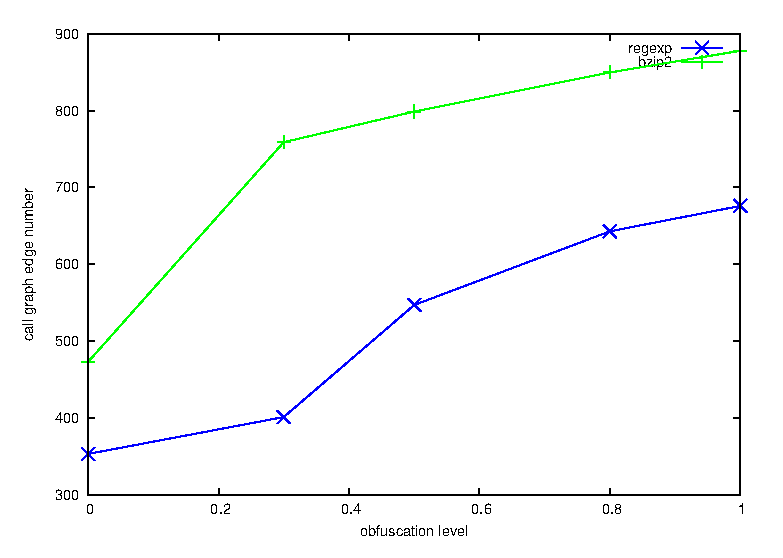
\includegraphics[width=0.9\linewidth]{cg.eps}
  \caption{Number of Call graph edges in terms of different obfuscation levels.}
  \label{fig:seven}
\end{figure}

\subsection{Resilience}
\label{subsec:resilience}
A good obfuscation technique should resist deobfuscation tools as well. Concolic
testing is an advanced deobfuscation technique aiming at finding bugs or
vulnerabilities in software through the mixture of symbolic execution and
concrete execution. Whereas, it is also used by adversaries to analyze or
restore software inner logic control flow graph\cite{Cadar,Sen,Cute}. KLEE~\cite{klee} is static analysis
tool based on LLVM platform and it could generate enough test cases to ensure a
code coverage threshhold. With the help of KLEE, it would be easy to conduct
automated deobfuscation by concolic testing. We chose KLEE as the deobfuscation
tool to evaluation resilience of Turing Machine obfuscator. We used a piece of
sample code from KLEE~\cite{klee} as the subject program (the sample code is
shown in \F~\ref{fig:klee-sample}). The subject program need to be converted to
IR codes since KLEE works on IR level.

\begin{figure}[h]
\centering
\begin{lstlisting}
    int get_sign(int x) {
      if (x == 0)
        return 0; 

      if (x < 0)
        return -1;
      else 
        return 1;
    }

    int main() {
      int a;
      klee_make_symbolic(&a, sizeof(a), "a");
      return get_sign(a);
    }
\end{lstlisting}
\caption{KLEE sample code used in our evaluation. All the path conditions are obfuscated.}
\label{fig:klee-sample}
\end{figure}


KLEE could detect three paths in the original subject program as expected. Based
on different value of x, this program may traverse branches in which x equals 0,
x is less than 0 and x is greater than 0, repectively. In contrast, after
subject program is obfuscated by our Turing machine obfuscator, KLEE could only
figure out one path. We interpret the evaluation result that Turing machine
obfuscator can impede automated deobfuscation tools from restoring the structure
of a program.

Due to limited information released by KLEE, we could not figure out the
underlying reason that leads the failure of KLEE. Since Turing machine
obfuscator make the conditional branches more complicated, our guess is that the
internal constraint solver employed by KLEE is unable to yield proper symbolic
input which ``drill'' into the branches protected by our Turing machine
obfuscator.


\subsection{Stealth}
As mentioned in the beginning, software obfuscation technique should not only
combat automated deobfuscation tools, but also manual deobfuscation methods. In
the evaluation of stealth, \cite{Trans} compares the instruction distributions
of original and obfuscated programs. If instruction distribution of the
obfuscated program is distinguishable from its original program (e.g
\texttt{call} or \texttt{jmp} instruction proportions are abnormally high), it
would be an obvious indicator that the program is manipulated. We adopted this
metric to evaluate our Turing obfuscator. Obfuscation level for stealth
evaluation is set to 50\%.

\begin{figure}
  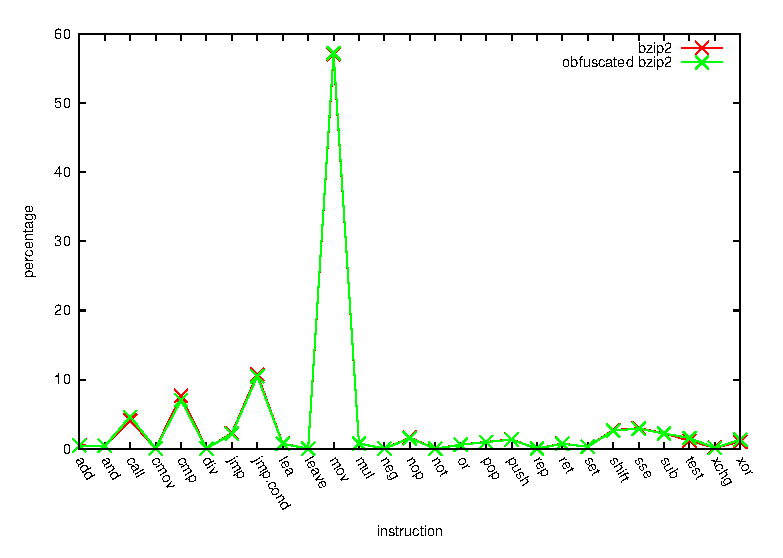
\includegraphics[width=0.9\linewidth]{st_bzip2.eps}
  \caption{\textsc{bzip2} instruction distribution comparison}
  \label{fig:bzip2}
\end{figure}

\begin{figure}
  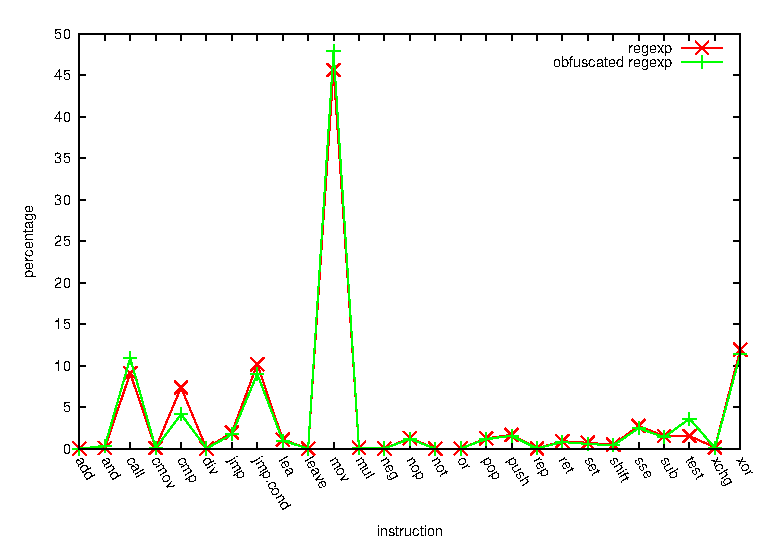
\includegraphics[width=0.9\linewidth]{st_regexp.eps}
  \caption{regexp instruction distribution comparison}
  \label{fig:regexp}
\end{figure}

Consistent with previous research (\cite{Trans}), we put assembly instructions
into 27 different categories. \F~\ref{fig:bzip2} and \F~\ref{fig:regexp} present
the instruction distribution of the original and obfuscated programs
(\textsc{bzip2} and \textsc{regexp}). Experiment results indicate that the
instruction distribution after obfuscation is very close to the origin
distribution. Comparing these two figures together, we noticed that instruction
diststribution variance of \textsc{regexp} is bigger than \textsc{bzip2}, it makes sense
since \textsc{regexp} consists of 8117 lines of Code and \textsc{regexp} contains only 1391 lines
of C code. In sum,
small instruction distribution variation is a promising result to show the
proposed technique would obfuscate programs in a stealthy way.

\subsection{Cost}
Software running cost is another critical factor in evaluating an obfuscation
technique. In most obfuscation research work, execution cost is inevitably
increased because obfuscation would bring in extra instructions. Measuring the
execution time is a convincing way to evaluate to the cost.

In our evaluation, both original and obfuscated programs are executed on a
server with 2 Intel(R) Xeon(R) E5-2690 2.90GHz processors and 128GB system
memory. \textsc{bzip2} is used to compress three different sample files and
regular expression engine \textsc{slre} runs 149 test cases provided by its
shipped test cases. We ran each program three times and recorded the average
time cost as the final result.

\begin{figure}
  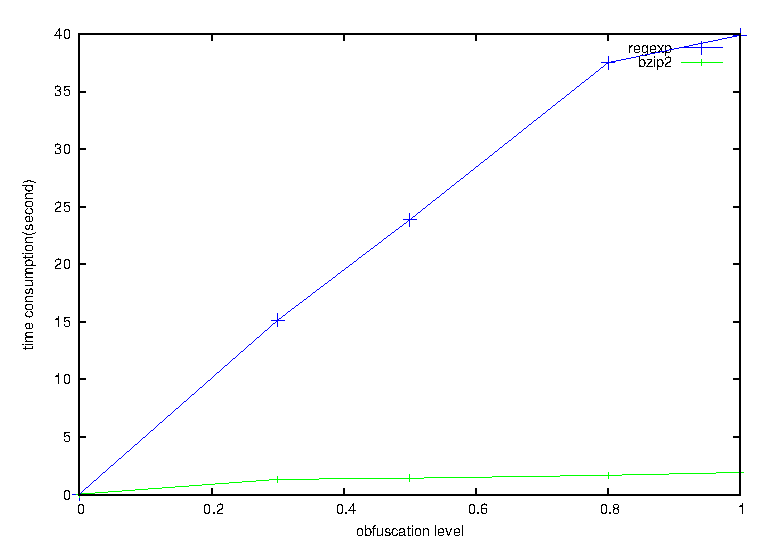
\includegraphics[width=0.9\linewidth]{cost.eps}
  \caption{Execution overhead in terms of different obfuscation levels.}
  \label{fig:cost}
\end{figure}

\F~\ref{fig:cost} shows that for both test cases, the execution slowly grows
w.r.t the increase of obfuscation levels. As expected, program takes more time
to execute with more instructions are obfuscated. On the other hand, we
interpret the overall time cost is still confined to a reasonable level. We also
notice that there exists a difference between slopes of the two curves. Turing
obfuscator randomly obfuscates candidate instructions within the program before
execution. Hence the transformed instructions may not be indeed executed in the
runtime. Difference between two curve slopes is probably due to such uncertainty
of execution. In addition, the regexp program employs more recursive calls than
\textsc{bzip2}, thus may contribute to the relatively higher cost grow as well.



\section{Discussion}
\label{sec:discussion}
To provide more insights and guideline for further adoption of our proposed
technique, we discuss the multiple aspects of the proposed Turing machine
technique in this section.

\subsection{Complexity}
In general, Turing machine model is a powerful calculator that is capable of
solving any algorithm problem. Note that even a simple operation (e.g., ``add'')
may lead to the change of Turing machine states for hundreds of times; every
``move left'' and ``move right'' operation lead to the tape modification and
``read'' or ``write'' operations.

Considering Turing machine as a state machine, it is hard---if possible at
all---for adversaries with manual reverse engineering to follow the calculation
logic without understanding the transition table rules and state variables. In
addition, the intrinsic Turing machine complexity can also defeat automated
deobfuscation tools (e.g., KLEE). As reported in our resilience evaluation
(\S~\ref{subsec:resilience}), the constraint solver of KLEE failed to yield
proper inputs to cover two of three execution paths.

\subsection{Application Scope}
Previous obfuscation work~\cite{Sharif} usually targets one or several specific
kinds of predicate expressions. Also, most of them performs source code level
transformations for specific kind of program languages~\cite{Trans}. Turing
obfuscator broadens the application scope to any kind of conditional expression.
In addition, it works for programs written in any language as long as they could
be transformed into the LLVM IR. Considering a large portion of programming
languages have been supported by LLVM, we envision Turning machine obfuscator
would serve to harden many softwares implemented with various kinds of
programming languages.

\subsection{Branch Selection Techniques}
As previously presented, our current implementation rewrites path condition
instructions to invoke the Turing machine component. While it is mostly
impossible for attackers to reason the functionality of the Turing machine code,
return value of executing the Turing machine component is observable (since the
predicate computation is modeled as a function call to the Turing machine
component). Certain amount of information leakage may become feasible at this
point.

We notice that existing work (\cite{Ma, Maieee}) proposes a different approach
at this step; control flow is directly guided (via \texttt{goto}) to the
selected branch from the Neural network obfuscator. While intuitively this
approach seems to hide the explicit return value, such approach is not
fundamentally more secure since the hidden return value can be inferred by
observing the execution flow. Another solution that may be employed to protect
the predicate computation result is to use matrix branch logic~\cite{Samjam}.
Suppose we model a branch predicate with a Turing machine function (e.g., $TM$),
the general idea is to further transform $TM$ into a matrix function, then
randomize the matrix branching function. The involved matrix branch logic and
randomness shall provide additional security consideration at this step.
Overall, we argue the current implementation is reasonable, and we leave it as
one future work to present quantitative analysis of the potential information
leakage and countermeasures at this step.

\subsection{Execution Overhead}
During the Turing machine computation, frequent state change would indicate lots
of read and write operations. Also, since tape is infinite in Turing machine
model, it needs to allocate enough memory to accommodate complex computations.
In general, the complexity of Turing machine is a double edge sword; it impedes
adversaries and increases execution overhead at the same time. As reported in
the cost evaluation (Fig.~\ref{fig:cost}), we observed non-negligible
performance penalty for both cases. One solution is to perform selective
obfuscation; users can mark sensitive program codes and Turing machine
obfuscator would only harden those parts. Such strategy would improve the
overall execution speed without sacrificing the major security requirements.

\section{Conclusion}
In this paper we proposed a novel obfuscation technique taking advantage of the
merits of Turing machine execution. We designed a prototype called Turing
machine obfuscator will LLVM platform. We implmented Turing machine and
universal Turing machine for arithmetic operators $+, -, *$ and $\div$. Return
value of Universal Turing machine execution is used to direct control flow. We
evaluated Turing machine obfuscator with respect to pontency, resilience,
stealth and cost with two open source software as subjects. Evaluation results
indicated effectiveness and robustness of Turing machine obfuscator. We believe
Turing machine obfuscator could be a solid and pratical obfuscation tool to
protect software security.


%
% ---- Bibliography ----
%
\begin{thebibliography}{5}

\bibitem{Sen} Sen, Koushik, Darko Marinov, and Gul Agha. "CUTE: a concolic unit testing engine for C." ACM SIGSOFT Software Engineering Notes. Vol. 30. No. 5. ACM, 2005.

\bibitem{Ma} Haoyu Ma, Xinjie Ma, Weijie Liu, Zhipeng Huang, Debin Gao and Chunfu Jia. "Control flow obfuscation using neural network to fight concolic testing." International Conference on Security and Privacy in Communication Systems. Springer International Publishing, 2014.

\bibitem{Trans} Pei Wang, Shuai Wang, Jiang Ming, Yufei Jiang, Dinghao Wu. "Translingual obfuscation." Security and Privacy (EuroS\&P), 2016 IEEE European Symposium on. IEEE, 2016.

\bibitem{Collberg} Collberg, Christian, Clark Thomborson, and Douglas Low. "Manufacturing cheap, resilient, and stealthy opaque constructs." Proceedings of the 25th ACM SIGPLAN-SIGACT symposium on Principles of programming languages. ACM, 1998.

\bibitem{Sharif} Sharif, Monirul I., et al. "Impeding Malware Analysis Using Conditional Code Obfuscation." NDSS. 2008.


\bibitem{SingleTape} \url{http://turingmaschine.klickagent.ch/}

\bibitem{Popov} Popov, Igor V., Saumya K. Debray, and Gregory R. Andrews. "Binary Obfuscation Using Signals." Usenix Security. 2007.

\bibitem{Zhi} Zhi Wang, Chunfu Jia, Min Liu. "Branch obfuscation using code mobility and signal." Computer Software and Applications Conference Workshops (COMPSACW), 2012 IEEE 36th Annual. IEEE, 2012.

\bibitem{Wang:Zhi} Zhi Wang, Jiang Ming, Chunfu Jia, Debin Gao. "Linear obfuscation to combat symbolic execution." European Symposium on Research in Computer Security. Springer Berlin Heidelberg, 2011.

\bibitem{bzip2} \url{http://www.bzip.org/}

\bibitem{slre} \url{https://github.com/cesanta/slre}

\bibitem{Chen} Chen, Haibo, et al. "Control flow obfuscation with information flow tracking." Proceedings of the 42nd Annual IEEE/ACM International Symposium on Microarchitecture. ACM, 2009.

\bibitem{ida} \url{https://www.hex-rays.com/products/ida/}

\bibitem{McCabe} McCabe, Thomas J. "A complexity measure." IEEE Transactions on software Engineering 4 (1976): 308-320.

\bibitem{Woodward} Woodward, Martin R., Michael A. Hennell, and David Hedley. "A measure of control flow complexity in program text." IEEE Transactions on Software Engineering 1 (1979): 45-50.

\bibitem{Turing} \url{https://en.wikipedia.org/wiki/Turing_machine}

\bibitem{Sage} Godefroid, Patrice, Michael Y. Levin, and David A. Molnar. "Automated Whitebox Fuzz Testing." NDSS. Vol. 8. 2008.

\bibitem{UTM} \url{https://en.wikipedia.org/wiki/Universal_Turing_machine#/media/File:Universal_Turing_machine.svg}

\bibitem{LLVM} \url{https://en.wikipedia.org/wiki/LLVM}

\bibitem{klee} \url{https://klee.github.io/}

\bibitem{Opaque} Xu, Dongpeng, Jiang Ming, and Dinghao Wu. "Generalized Dynamic Opaque Predicates: A New Control Flow Obfuscation Method." International Conference on Information Security. Springer International Publishing, 2016.

\bibitem{Loop} Ming, Jiang, et al. "Loop: Logic-oriented opaque predicate detection in obfuscated binary code." Proceedings of the 22nd ACM SIGSAC Conference on Computer and Communications Security. ACM, 2015.

\bibitem{Lee} Lee, Gareth, et al. "Using symbolic execution to guide test generation." Software Testing, Verification and Reliability 15.1 (2005): 41-61.

\bibitem{Molnar} Molnar, David, Xue Cong Li, and David Wagner. "Dynamic Test Generation to Find Integer Bugs in x86 Binary Linux Programs." USENIX Security Symposium. Vol. 9. 2009.

\bibitem{Church} \url{https://en.wikipedia.org/wiki/Church%E2%80%93Turing_thesis}

\bibitem{llvmpass} \url{http://llvm.org/docs/WritingAnLLVMPass.html}

%\bibitem{Sen} Sen, Koushik, Darko Marinov, and Gul Agha. "CUTE: a concolic unit testing engine for C." ACM SIGSOFT Software Engineering Notes. Vol. 30. No. 5. ACM, 2005.

\bibitem{Cute} Sen, Koushik, and Gul Agha. "CUTE and jCUTE: Concolic unit testing and explicit path model-checking tools." International Conference on Computer Aided Verification. Springer Berlin Heidelberg, 2006.

\bibitem{Cadar} Cadar, Cristian, Daniel Dunbar, and Dawson R. Engler. "KLEE: Unassisted and Automatic Generation of High-Coverage Tests for Complex Systems Programs." The 11st USENIX Symposium on Operating Systems Design and Implementation (OSDI). 2008.

\bibitem{Samjam} Garg, Sanjam and Gentry, Craig and Halevi, Shai and Raykova, Mariana and Sahai, Amit and Waters, Brent. ``Candidate Indistinguishability Obfuscation and Functional Encryption for All Circuits.'' The 53rd Annual Symposium on Foundations of Computer Science (FOCS). 2013.

\bibitem{Maieee} Hanoyu Ma, Ruiqi Li, Xiaoxu Yu, Chunfu Jia, Debin Gao. ``Integrated Software Fingerprinting via Neural-Network-Based Control Flow Obfuscation.'' IEEE Transactions on Information Forensics \& Security (TIFS). 2016.

\end{thebibliography}
%
\end{document}
